%
% Main document
% ===========================================================================
\documentclass[
    paper=a4,               % paper format
    fontsize=10pt,          % fontsize
    %twoside,               % double-sided
    open=right,             % begin new chapter on right side
    titlepage=false,        % use no standard title page
    parskip=half,           % set paragraph skip to half of a line
]{scrreprt}                 % KOMA-script report
%---------------------------------------------------------------------------
\raggedbottom{}
%\KOMAoptions{cleardoublepage=plain}                                    % Add header and footer on blank pages


% Load Standard Packages:
%---------------------------------------------------------------------------
\usepackage[standard-baselineskips]{cmbright}

\usepackage{scrhack}
\usepackage[ngerman]{babel}                                             % german hyphenation
\usepackage[utf8]{inputenc}                                             % UTF-8 character encoding
\usepackage[T1]{fontenc}                                                % hyphenation of words with ä,ö and ü
\usepackage{textcomp}                                                   % additional symbols
\usepackage{ae}                                                         % better resolution of Type1-Fonts 
% \usepackage{fancyhdr}                                                   % simple manipulation of header and footer 
\usepackage{etoolbox}                                                   % color manipulation of header and footer
\usepackage{graphicx}                                                   % integration of images
\usepackage{float}                                                      % floating objects
\usepackage{caption}                                                    % for captions of figures and tables
\usepackage{booktabs}                                                   % package for nicer tables
\usepackage{tocvsec2}                                                   % provides means of controlling the sectional numbering
\usepackage[square,sort,comma,numbers]{natbib}                          % provides various citation styles
\usepackage{wrapfig}                                                    % provides floating of text around images
\usepackage{nameref}                                                    % provides printing names of references
%---------------------------------------------------------------------------

% Definition of Colors
%---------------------------------------------------------------------------
\RequirePackage{color}                                                  % Color (not xcolor!)
\definecolor{linkblue}{rgb}{0,0,0.8}                                    % Standard
\definecolor{darkblue}{rgb}{0,0.08,0.45}                                % Dark blue
\definecolor{bfhgrey}{rgb}{0.41,0.49,0.57}                              % BFH grey
%\definecolor{linkcolor}{rgb}{0,0,0.8}                                  % Blue for the web- and cd-version!
\definecolor{linkcolor}{rgb}{0,0,0}                                     % Black for the print-version!
\definecolor{codecommentcolor}{rgb}{0, 0.6, 0}                          % Color for code comments
\definecolor{black}{rgb}{0, 0, 0}
\definecolor{maroon}{rgb}{0.5,0,0}
\definecolor{darkgreen}{rgb}{0,0.5,0}
\definecolor{darkblue}{rgb}{0.0,0.0,0.6}
%---------------------------------------------------------------------------

% Load listings package
% which provides source code formatting
%---------------------------------------------------------------------------
\usepackage{listings}                                                   % provides source code formatting
% Define XML colors
\lstdefinelanguage{XML}
{basicstyle=\ttfamily\footnotesize,
  morestring=[b]'',
  moredelim=[s][\bfseries\color{maroon}]{<}{\ },
  moredelim=[s][\bfseries\color{maroon}]{</}{>},
  moredelim=[l][\bfseries\color{maroon}]{/>},
  moredelim=[l][\bfseries\color{maroon}]{>},
  morecomment=[s]{<?}{?>},
  morecomment=[s]{<!--}{-->},
  commentstyle=\color{codecommentcolor},
  stringstyle=\color{darkblue},
  identifierstyle=\color{red}
}
%---------------------------------------------------------------------------

% Comment package
%---------------------------------------------------------------------------
\usepackage{comment}
%---------------------------------------------------------------------------

% Load Math Packages
%---------------------------------------------------------------------------
\usepackage{amsmath}                                                    % various features to facilitate writing math formulas
\usepackage{amsthm}                                                     % enhanced version of latex's newtheorem
\usepackage{amsfonts}                                                   % set of miscellaneous TeX fonts that augment the standard CM
\usepackage{amssymb}                                                    % mathematical special characters
\usepackage{exscale}                                                    % mathematical size corresponds to textsize
%---------------------------------------------------------------------------

% Package to facilitate placement of boxes at absolute positions
%---------------------------------------------------------------------------
\usepackage[absolute]{textpos}
\setlength{\TPHorizModule}{1mm}
\setlength{\TPVertModule}{1mm}
%---------------------------------------------------------------------------

% Package for annotations
% See http://ctan.mirrorcatalogs.com/macros/latex/contrib/ed/ed.pdf
%---------------------------------------------------------------------------
\usepackage[hide]{ed}
%---------------------------------------------------------------------------

% Hyperref Package (Create links in a pdf)
%---------------------------------------------------------------------------
\usepackage[
    pdftex,ngerman,bookmarks,plainpages=false,pdfpagelabels,
    backref = {false},                                                  % No index backreference
    colorlinks = {true},                                                % Color links in a PDF
    hypertexnames = {true},                                             % no failures "same page(i)"
    bookmarksopen = {true},                                             % opens the bar on the left side
    bookmarksopenlevel = {0},                                           % depth of opened bookmarks
    pdftitle = {Erkennung von aktiven Konturen mittels Matlab},                          % PDF-property
    pdfauthor = {brd3},                                                 % PDF-property
    pdfsubject = {Projektarbeit},                                      % PDF-property
    linkcolor = {linkcolor},                                            % Color of Links
    citecolor = {linkcolor},                                            % Color of Cite-Links
    urlcolor = {linkcolor},                                             % Color of URLs
]{hyperref}
%---------------------------------------------------------------------------

% Cross-reference package
%---------------------------------------------------------------------------
\usepackage{xr}                                                         % provides references to other, external documents
%---------------------------------------------------------------------------
% Set up page dimension
%---------------------------------------------------------------------------
\usepackage{geometry}
\geometry{a4paper,
    left=28mm,
    right=15mm,
    top=30mm,
    headheight=20mm,
    headsep=10mm,
    textheight=242mm,
    footskip=15mm
}
%---------------------------------------------------------------------------

% Makeindex Package
%---------------------------------------------------------------------------
\usepackage{makeidx}                                % To produce index
\makeindex                                      % Index-Initialisation
%---------------------------------------------------------------------------

% Glossary Package
%---------------------------------------------------------------------------
% the glossaries package uses makeindex
% if you use TeXnicCenter do the following steps:
%  - Goto "Ausgabeprofile definieren" (ctrl + F7)
%  - Select the profile "LaTeX => PDF"
%  - Add in register "Nachbearbeitung" a new "Postprozessoren" point named Glossar
%  - Select makeindex.exe in the field "Anwendung" ( ..\MiKTeX x.x\miktex\bin\makeindex.exe )
%  - Add this [ -s "%tm.ist" -t "%tm.glg" -o "%tm.gls" "%tm.glo" ] in the field "Argumente"
%
% for futher informations go to http://ewus.de/tipp-1029.html
%---------------------------------------------------------------------------
\usepackage[nonumberlist]{glossaries}
\makeglossaries{}
\newglossaryentry{aktiver Konturen}
{
    name=Aktive Konturen,
    description={Foos the bar}
}

\newglossaryentry{Segmentationsmethoden}
{
    name=Segmentation,
    description={``Segmentieren beduetet, jedes Pixel einer bestimmten Region zuzuweisen.''~\cite[S. 133]{hudritsch:script:cp}}
}

%---------------------------------------------------------------------------

% Intro:
%---------------------------------------------------------------------------
%\begin{document}                                % Start Document
\settocdepth{section}                                                       % Set depth of toc
\pagenumbering{roman}                                                       
%---------------------------------------------------------------------------

\providecommand{\title}{Erkennung von aktiven Konturen mittels Matlab}
                  % Titel der Arbeit aus Datei titel.tex lesen
% Current version number
\providecommand{\versionnumber}{0.5}

% Date of the current version
\providecommand{\versiondate}{{\today}}
                % Versionsnummer und -datum aus Datei version.tex lesen

% Set up header and footer
%---------------------------------------------------------------------------
% \makeatletter
% \patchcmd{\fancyhead}{\rlap}{\color{bfhgrey}\rlap}{}{}     % new color of header
% \patchcmd{\fancyfoot}{\rlap}{\color{bfhgrey}\rlap}{}{}     % new color of footer
% \makeatother
% 
% \fancyhf{}                                                                      % clean all fields
% \fancypagestyle{plain}{% new definition of plain style 
%     \fancyfoot[OR,EL]{\footnotesize \thepage}   % footer right part --> page number
%     \fancyfoot[OL,ER]{\footnotesize \titel, Version \versionnumber, \versiondate}   % footer even page left part 
% }

% \renewcommand{\chaptermark}[1]{\markboth{\thechapter.  #1}{}}
% \renewcommand{\headrulewidth}{0pt}              % no header stripline
% \renewcommand{\footrulewidth}{0pt}              % no bottom stripline

% Randnotizen
\newcommand\mpar[1]{\marginpar{\flushleft\sffamily\small #1}}
\setlength{\marginparwidth}{1.5cm}

\pagestyle{plain}
%---------------------------------------------------------------------------

\begin{document}

\lstset{language=XML,
  caption={},
  frame=L,
  basicstyle=\small\normalfont\sffamily,  % the size of the fonts that are used for the code
  stepnumber=1,                           % the step between two line-numbers.
                                          % If it is 1 each line will be numbered
  numbersep=10pt,                         % how far the line-numbers are from the code
  tabsize=2,                              % tab size in blank spaces
  extendedchars=true,                     %
  breaklines=true,                        % sets automatic line breaking
  captionpos=b,                           % sets the caption-position to bottom
  mathescape=true,
  showspaces=false,                       % Leerzeichen anzeigen ?
  showtabs=false,                         % Tabs anzeigen ?
  xleftmargin=17pt,
  framexleftmargin=17pt,
  framexrightmargin=17pt,
  framexbottommargin=5pt,
  framextopmargin=5pt,
  showstringspaces=false                  % Leerzeichen in Strings anzeigen ?
  belowcaptionskip=5em,
  belowskip=3em,
  aboveskip=3em
 }

% Make sure Umlauts are getting displayed correctly.
\lstset{literate=%
    {Ö}{\textcolor{red}{\"O}}1
    {Ä}{{\"A}}1
    {Ü}{{\"U}}1
    {ß}{{\ss}}1
    {ü}{{\"u}}1
    {ä}{{\textcolor{red}{\"a}}}1
    {ö}{{\textcolor{red}{\"o}}}1
    {~}{{\textasciitilde}}1
    {?}{{\textcolor{red}{?}}}1
}

% Title Page and Abstract
%---------------------------------------------------------------------------
\begin{titlepage}

\setlength{\unitlength}{1mm}
\begin{textblock}{20}[0,0](28,12) % chktex-file 36
    
\includegraphics[scale=1.0]{images/BFH_Logo_B.png}
\end{textblock}

\begin{textblock}{154}(28,48)
    \begin{picture}(150,2)
        \put(0,0){\color{bfhgrey}\rule{150mm}{2mm}}
    \end{picture}
\end{textblock}

\begin{textblock}{154}[0,0](26.7,50.5)
    \centering
    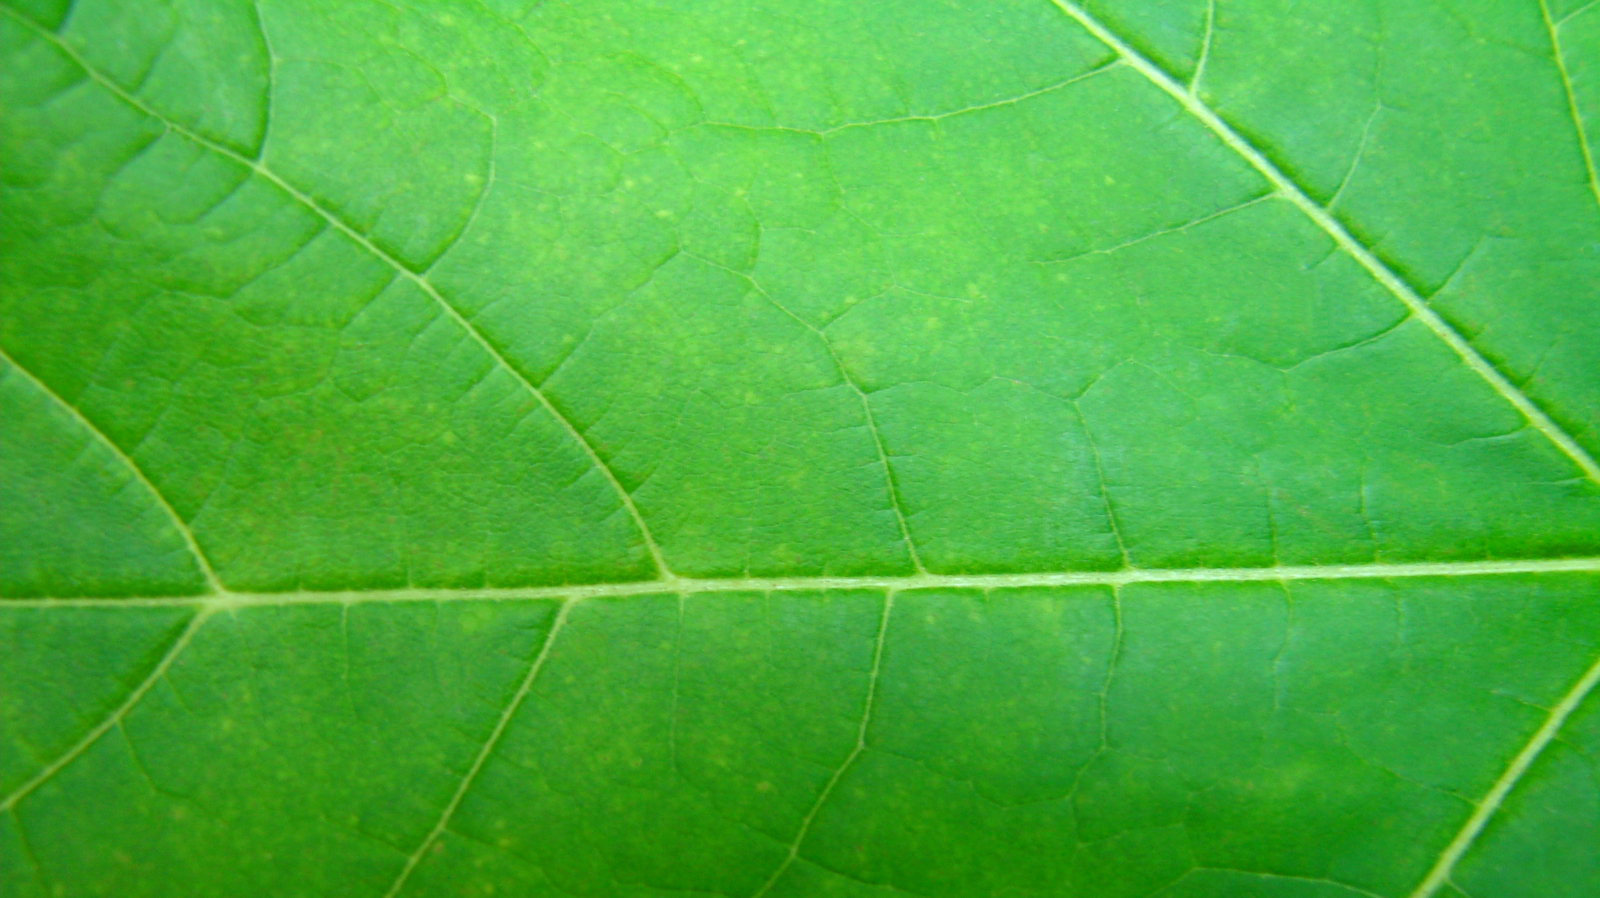
\includegraphics[scale=0.264]{images/title.jpg}\protect\footnotemark{}
\end{textblock}
\footnotetext{Quelle: \url{http://www.freeimages.com/photo/1358335}}

\begin{textblock}{154} (28,135)
    \begin{picture}(150,2)
        \put(0,0){\color{bfhgrey}\rule{150mm}{2mm}}
    \end{picture}
\end{textblock}
\color{black}

\begin{flushleft}

\vspace*{120mm}

\fontsize{26pt}{28pt}\selectfont
Erkennung von aktiven Konturen mittels Matlab
\vspace{3mm}

\fontsize{20pt}{22pt}\selectfont
Projektarbeit
\vspace{3mm}

\fontsize{10pt}{12pt}\selectfont
\textbf{BZG1301: Programmierung mit Matlab/Octave} \\
\vspace{3mm}

\begin{textblock}{150} (28,215)
\fontsize{10pt}{17pt}\selectfont
\begin{tabbing}
xxxxxxxxxxxxxxx\=xxxxxxxxxxxxxxxxxxxxxxxxxxxxxxxxxxxxxxxxxxxxxxx \kill
Autor:        \> Sven Osterwalder\\
Datum:        \> \versiondate\\
Betreuer:     \> Marx Stampfli\\
\end{tabbing}

\end{textblock}
\end{flushleft}

\begin{textblock}{150} (28,280)
\noindent 
\color{bfhgrey}\fontsize{9pt}{10pt}\selectfont
Berner Fachhochschule | Haute école spécialisée bernoise | Bern University of Applied Sciences
\color{black}\selectfont
\end{textblock}


\end{titlepage}

\cleardoublepage{}
\phantomsection{}
\chapter*{}
\label{chap:versionen}

\begin{textblock}{180} (15,150)
\color{black}
\begin{huge}
Versionen
\end{huge}
\vspace{10mm}

\fontsize{10pt}{18pt}\selectfont
\begin{tabbing}
xxxxxxxxxxx\=xxxxxxxxxxxxxxx\=xxxxxxxxxxxxxx\=xxxxxxxxxxxxxxxxxxxxxxxxxxxxxxxxxxxxxxxxxxxxxxx \kill
\textit{Version}	\> \textit{Kalenderwoche}	\> \textit{Status}		\> \textit{Bemerkungen}\\
0.1	\> 9	\> Entwurf		\> Initiale Erstellung des Dokuments\\
0.2	\> 10	\> Entwurf		\> Erstellung Konzept\\
0.3	\> 11	\> Entwurf		\> Verfassen der Einleitung und Grundlagen\\
\end{tabbing}

\end{textblock}

\phantomsection{}
\cleardoubleemptypage{}
\setcounter{page}{1}
\cleardoublepage{}
\phantomsection{}
%\addcontentsline{toc}{chapter}{Versionen}
\cleardoubleemptypage{}
%---------------------------------------------------------------------------

% Table of contents
%---------------------------------------------------------------------------
\tableofcontents
\cleardoublepage{}
%---------------------------------------------------------------------------

% Main part:
%---------------------------------------------------------------------------
\pagenumbering{arabic}
\chapter{Einführung}
\label{chap:intro}

%---------------------------------------------------------------------------

% Glossary
%---------------------------------------------------------------------------
\cleardoublepage{}
\phantomsection{}
\addcontentsline{toc}{chapter}{Glossar}
\renewcommand{\glossaryname}{Glossar}
\printglossary{}
%---------------------------------------------------------------------------

% Bibliography
%---------------------------------------------------------------------------

\phantomsection{}
\addcontentsline{toc}{chapter}{Literaturverzeichnis}
\bibliographystyle{unsrtnat}
%\bibliography{db/bibliography}{}
%---------------------------------------------------------------------------

% Listings
%---------------------------------------------------------------------------

\phantomsection{}
\addcontentsline{toc}{chapter}{Abbildungsverzeichnis}
\listoffigures

%\phantomsection{}
%\addcontentsline{toc}{chapter}{Tabellenverzeichnis}
%\listoftables
%---------------------------------------------------------------------------

% Index
%---------------------------------------------------------------------------

%\phantomsection{}
%\addcontentsline{toc}{chapter}{Stichwortverzeichnis}
%\renewcommand{\indexname}{Stichwortverzeichnis}
%\printindex
%---------------------------------------------------------------------------

% Attachment:
%---------------------------------------------------------------------------
\appendix
\settocdepth{section}
%\include{anhang/beispielanhang}
%---------------------------------------------------------------------------

%---------------------------------------------------------------------------
\end{document}
